The counterexamples for general surveillance properties are directed graphs, which may contain cycles. In particular, for a liveness surveillance property of the form $\LTLglobally\LTLfinally p_k$ each infinite path in the graph contains has a position such that, from this position on each state on the path violates $p_k$. Formally, an \emph{abstract counterexample graph} for the abstract game $(G_\abstr,\LTLglobally\LTLfinally p_k)$ is a finite graph $\counterex_\abstr$ such that:
\begin{itemize}
\item There exists a node $v_0$ of $\counterex_\abstr$ labelled with $s^\init_\abstr$.
\item For each cycle $\rho = v_1,v_2,\ldots,v_n$ with $v_1 = v_n$ in $\counterex_abstr$ that is reachable from $v_0$, every node $v_i$ in $\rho$ is labelled with state $s_\abstr^i$ where $s_\abstr^i \not\models s_\abstr^i$.
\item The tree branches according to all possible transition choices of the agent. Formally, if an internal node $v$ is labelled with $(l_a,A_t)$, then there exists an $A_t'$  such that: (1) $((l_a,A_t),(l_a',A_t')) \in \trans_\abstr$ for some $l_a' \in L_a$, and (2) for every $l_a' \in L_a$ such that $((l_a,A_t),(l_a,A_t')) \in \trans_\abstr$, there is a child $v'$ of $v$ labelled with $(l_a',A_t')$.
\end{itemize}   

\begin{figure}
\begin{center}
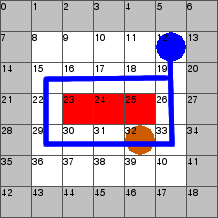
\includegraphics[scale=.33]{figs/7x7_liveness.png}
\end{center}
\caption{Agent locations on an (infinite) path in the abstract counterexample graph from Example~\ref{ex:simple-liveness-counterex}. In the counterexample graph, the first node is labelled with $(12,32)$, the second with $(19,\{Q_2\})$, and all other nodes with $(19,\{Q_1,Q_2\})$.}
\label{fig:simple-liveness-counterex}
\end{figure}

\begin{example}\label{ex:simple-liveness-counterex}
As we saw in Example~\ref{ex:simple-safety-realizability}, in the safety surveillance game $(G,\LTLglobally p_2)$ the agent does not have a winning strategy. This means, that the agent cannot ensure keeping at all times the uncertainty about the current position of the target to at most two positions.

We now consider a more relaxed requirement, namely that the uncertainty drops to at most two infinitely often. Formally, we consider the liveness surveillance game 
$(G,\LTLglobally \LTLfinally p_2)$.

Let $\part = \{Q_1,Q_2\}$ be the partition from Example~\ref{ex:simple-safety-unconcretizable},  that is, $Q_1$, corresponds to the first two columns of the grid in Figure~\ref{simple-grid} and the set $Q_2$ contains the locations from the other three columns of the grid. Figure~\ref{fig:simple-liveness-counterex} shows an infinite path (in lasso form) in the abstract game $(\alpha_\part(G),\LTLglobally \LTLfinally p_2)$.  The figure depicts only the corresponding trajectory (sequence of positions) of the agent. The initial abstract belief set is $(12,32)$, the second node on the path is labelled with the abstract state $(19,\{Q_2\})$, and all other nodes on the path are labelled with abstract states of the form $(l_a,\{Q_1,Q_2\})$. As each abstract state in the cycle violates the surveillance predicate $p_2$, the path violates $\LTLglobally \LTLfinally p_2$. The same holds for all infinite paths in the abstract counterexample graph.
\qed
\end{example}

A \emph{concrete counterexample graph} $\counterex_\belief$ for the belief game $(G_\belief,\LTLglobally\LTLfinally p_k)$ is defined analogously. 

An abstract counterexample graph $\counterex_\abstr$ for the game $(G_\abstr,\LTLglobally\LTLfinally p_k)$ is \emph{concretizable} if there exists a counterexample
$\counterex_\belief$ in $(G_\belief,\LTLglobally \LTLfinally p_k)$, such that for each infinite path $\pi_\abstr = n_\abstr^0,n_\abstr^1,\ldots$ starting from the initial node of $\counterex_\abstr$ there exists an infinite path $\pi_\belief = n_\belief^0,n_\belief^1,\ldots$ in $\counterex_\belief$ staring from its initial node such that if $n_\abstr^i$ is labelled with $(l_a,A_t)$ in $\counterex_\abstr$, then the corresponding node $n_\belief^i$ in $\counterex_\belief$ is labelled with $(l_a,B_t)$ for some $B_t \in \mathcal{P}(L_t)$ for which $B_t \subseteq \gamma(A_t)$.

